\chapter{А это что за штука? Устройство гитары}
\label{ch:guitar}

Гитара\index{гитара} --- простой и изящный музыкальный инструмент. Благодаря этим качествам ей и удалось завоевать сердца многих исполнителей.

Но не путайте простоту с безграмотностью! Гитара --- инструмент для извлечения звуков \emph{равномерно темперированного строя}. Вспомним (см. раздел \ref{ch:music:tone}), что строй --- это правила отбора частоты колебаний основного тона для особых звуков, которые называются \emph{музыкальными}. Именно такие звуки извлекают из \emph{музыкального} инструмента.

Так увидим же математику строя в конструкции гитары, а затем разберемся с тем, как правильно её на\emph{строить}.


\section{Может разберем? Конструкция}
\label{ch:guitar:construction}

Взглянем на рисунок \ref{fig:guitar:construction}, чтобы узнать, как называются отдельные части гитары.

\begin{figure}[!ht]
    \centering
    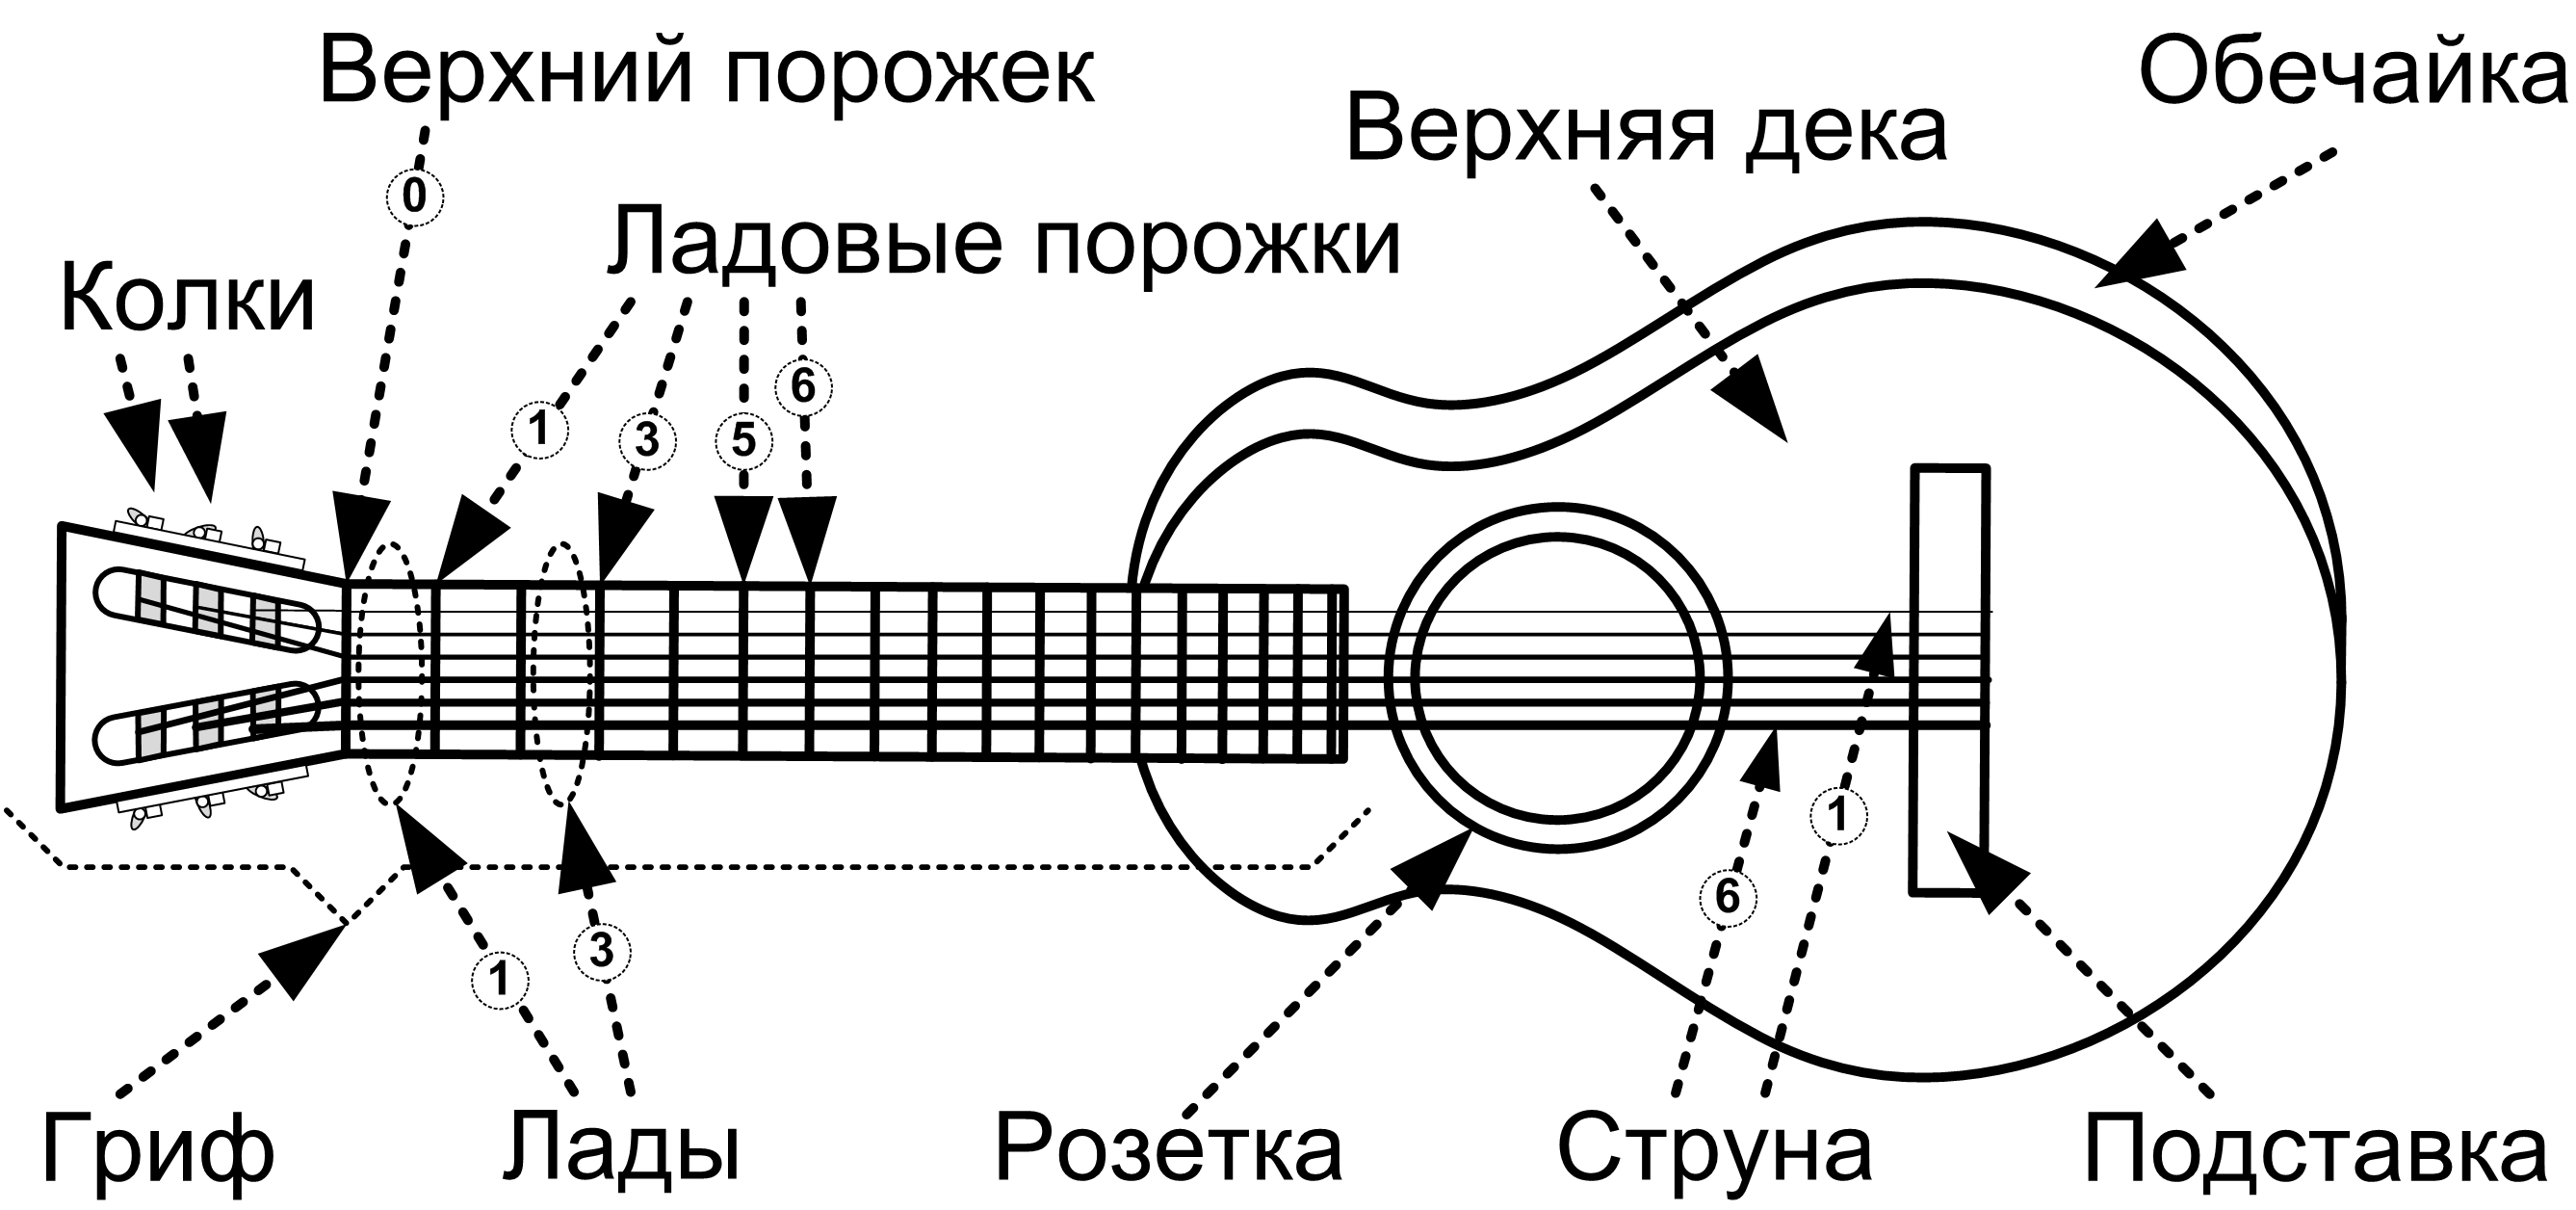
\includegraphics{fig/guitar-construction} 
    \caption{Устройство гитары\index{гитара!устройство}}\label{fig:guitar:construction}
\end{figure} 

Отдельная \emph{струна} одним концом крепится к неподвижной \emph{подставке}, а вторым концом наматывается на барабанчик \emph{колка}. Червячный механизм колка позволяет очень тонко регулировать степень натяжения струны. Струна натягивается вдоль \emph{грифа}, поперек которого врезаны на определенном расстоянии друг от друга металлические выступы --- \emph{ладовые порожки}. Струна натянута так, что её звучащая (колеблющаяся) часть опирается своими концами на верхний и нижний порожки, а остальных ладовых порожков не касается, хотя и проходит достаточно близко к ним\footnote{
    Приведу все же немного справочных данных о расстояниях\index{струна!высота над грифом} от струн до ладов. С одной стороны, чем оно меньше, тем легче и быстрее укорачивается струна, а с другой стороны, слишком <<зaниженная>> струна может во время игры начать звенеть, касаясь ладовых порожков. Для классической аккустической гитары (с нейлоновыми струнами) средние показатели такие: 
    \begin{itemize}
        \item расстояние от 1-й струны до 1-го ладового порожка составляет 0.61 мм, а до 12-го --- 3.18 мм;
        \item от 6-й струны до 1-го порожка --- 0.76 мм, а до 12-го --- 3.96 мм;
    \end{itemize}
    
    Для эстрадной аккустической гитары (со стальными струнами и анкерным стержнем внутри грифа) расстояния следующие:
    \begin{itemize}
        \item от 1-й струны до 1-го порожка --- 0.33 мм, а до 12-го --- 1.78 мм;
        \item от 6-й струны до 1-го порожка --- 0.58 мм, а до 12-го --- 2.29 мм;
    \end{itemize}
    
    Пусть вас не пугают приведенные с точностью до сотых долей миллиметра числа --- они являются расчетными. На практике регулировка осуществляется подтачиванием верхнего порожка и порожка на подставке. Замеры расстояния осуществляются (в порядке увеличения популярности): штангенциркулем, стальной слесарной линейкой, просто <<на глазок>> --- но никак не микрометром! У людей профессионально занимающихся доводкой гитар, обычно заготовлены пластинки нужной толщины, и высота контролируется простым просовыванием пластинки между струной и порожком.
    
    Единого стандарта на высоту струн нет. Профессионалы, естественно, занижают высоту струн до предела, чего новичкам делать не следует. С завода бюджетные гитары обычно поступают в магазины с <<завышенной>> высотой струн и требуют доводки. В хорошем музыкальном магазине либо <<доведут>> гитару при покупке, либо посоветуют гитарного мастера.
}

Известно, что частота колебаний струны зависит от степени её натяжения и её длины. Перед тем как играть, гитару \emph{настраивают}, то есть с помощью колков каждую струну натягивают так, чтобы она издавала строго определенный \emph{музыкальный} звук. Чем сильнее натянута струна, тем выше звук (т.е. тем больше частота колебаний струны). А уже играя, гитарист прижимает пальцем левой рукой струну к ладовому порожку, чем практически мгновенно укорачивает её звучащую часть. Что в свою очередь приводит к повышению звука, так как частота колебаний струны обратно пропорциональна её длине\footnote{Надо честно заметить, что частота колебаний струны зависит также и от силы её натяжения, которая меняется, когда струну <<зажимают>> на ладу. Но это влияние столь незначительно, что им можно пренебречь}.

Теперь давайте вспомним о самых важных музыкальных единицах измерения расстояния между двумя \emph{музыкальными} звуками.
\begin{itemize}
    \item \emph{Октава} --- звук $x$ \emph{выше} звука $y$ на \emph{октаву}, если частота колебаний основного тона звука $x$ больше частоты основного тона звука $y$ вдвое. Чтобы повысить звук открытой струны на октаву, нужно укоротить её вдвое, сохранив натяжение.
    
    \item \emph{Полутон} --- двенадцатая часть октавы. Теоретически неделимое расстояние между двумя музыкальными звуками. Звук $x$ \emph{выше} звука $y$ на \emph{полутон}, если частота основного тона звука $x$ больше частоты основного тона $y$ в $\sqrt[12]{2}$. Откуда квадратные корни? Проверьте: двенадцать раз повысив высоту звука $y$ на полутон, получим звук $x$ с частотой в $(\sqrt[12]{2})^{12}$ больше частоты исходного $y$. Так как $(\sqrt[12]{2})^{12} = 2$, то мы получили расстояние в октаву, что и требовалось! 
\end{itemize}


\begin{Definition}[Суть гитарной простоты]
    Номер лада на грифе гитары соответствует количеству \emph{полутонов}, на которое \emph{повышается} звук открытой струны, если её зажать на этом ладу.
\end{Definition}

Сдвинулись по грифу на лад --- повысили (или понизили) звук на \emph{полутон}. Сдвинулись на 12 ладов --- повысили/понизили на \emph{октаву}. И вообще: над 12 ладовым порожком находится середина струны!

В соотвествии с правилами равномерно темперированного строя (см. раздел \eqref{ch:music:tone}) частота основного тона струны зажатой на $n$-м ладу $f(n)$ будет определяться как 
\[
    f(n) = f_\text{откр}\cdot(\sqrt[12]{2})^n,
\] 
где $f_\text{откр}$ --- частота основного тона открытой струны. А так как частота колебаний струны обратно-пропорциональна её длине, то длина зажатой на $n$-м ладу струны $L(n)$, дающей звук нужной частоты, будет определяться так:

\begin{equation}
    \label{eq:guitar:construction:length}
    L(n) = \frac{L}{(\sqrt[12]{2})^n},
\end{equation}
где $n$ --- номер лада ($0$-й лад соответствует открытой струне, см. рисунок \ref{fig:guitar:construction}), а $L$ --- общая длина <<открытой>> струны: от подставки до верхнего порожка.

\begin{figure}[!ht]
    \centering
    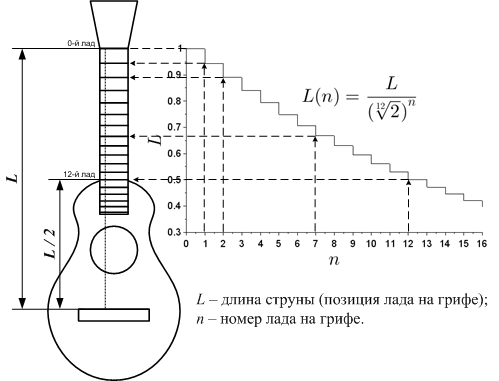
\includegraphics{fig/string-length.png}
    \caption{Расстояние между ладами}\label{fig:guitar:construction:length}
\end{figure} 

Вот и готова конструкция гитары! На рисунке \ref{fig:guitar:construction:length} соотнесён график функции \ref{eq:guitar:construction:length} с расположением ладов на гитарном грифе. Теперь ясно, например, почему по мере приближения к розетке расстояние между ладами становится всё меньше.

Кстати, некоторые ушастые выпендрёжники говорят, что различают своим сверхмузыкальным слухом больше 12 нот в октаве! Давайте делить полутон! Есть спрос --- есть предложение: на некоторых гитарах можно заметить дополнительные ладовые порожки между <<каноническими>>, которые позволяют <<всунуть>> дополнительную ноту.

Играя, гитарист лишь меняет длину звучащего участка струны, зажимая струны на ладах. Однако редкие психи/мастера крутят колок во время исполнения, добиваясь сомнительных/удивительных музыкальных эффектов.

Так, ядом поплевались, хорошо, хватит. Давайте закончим тему конструкции гитары чем-нибудь полезным. Например, выбирая гитару, стоит проверить, что она изготовлена по всем правилам\footnote{Сейчас нарваться в музыкальном магазине на нестроящую гитару --- случай редкий. Но всё же нельзя полностью исключать брак серийного производства. 3Б подход: Береженого --- Бог Бережет\ldots}. Музыканты скажут: проверить строй. Середина струны должна находиться точно над 12-м ладом, четверть (приблизительно) над 5-м ладом, треть (приблизительно) --- над 7-м. Проще всего это проверить без линейки, сыграв флажолеты, см. раздел \ref{ch:tricks:flageolet}. На <<нестр\'{о}ящей>> гитаре флажолеты не прозвучат.


\section{Правильно устроена? --- не значит, что настроена!}
\label{ch:guitar:tuning}

Начнём с того, что никогда, никогда, никогда\ldots \emph{НИКОГДА} не играйте на ненастроенном инструменте!

Продолжим тем, что настроить\index{гитара!настройка} гитару можно по-разному\index{строй!гитары}. Все зависит от того, как натянуть струны. И, строго говоря, этих вариантов много. Очень много. Но есть один, который любят все! И называется он: <<классический гитарный строй>>\index{строй!гитары!испанский}, он же <<испанский>>\index{строй!гитары!классический}, он же <<МИ>> (по-русски), он же <<E>>\footnote{E --- буква латинского алфавита. Используется для обозначения ноты МИ и произносится на русском как <<и>>. Учтите, что <<и>>-кать нужно только для иностранцев --- не злите Русских гитаристов}. 

Мы научимся настраивать гитару классическим строем. Именно он используется по умолчанию. Да он практически всегда используется! Увидели аппликатуры и табулатуры для шестиструнной гитары? --- в 99.9\% случаев они для классического строя. Для новичка уж точно выбора нет: сначала научись как все, а потом экспериментируй с настройкой гитары.

Итак, классический строй\footnote{Если не знаете, что такое ноты --- обратитьесь к разделу \ref{ch:notes}}.
\begin{itemize}
    \item МИ(E): первая струна настраивается колком на звук МИ \emph{первой} октавы.
    \item СИ(B): вторая струна настраивается на СИ \emph{малой} октавы.
    \item СОЛЬ(G): треться струна --- СОЛЬ \emph{малой} октавы.
    \item РЕ(D): четвертая --- МИ \emph{малой} октавы.
    \item ЛЯ(A): пятая --- ЛЯ \emph{большой} октавы.
    \item МИ(E): шестая --- МИ \emph{большой} октавы.
\end{itemize}

Неплохо бы запомнить последовательность: МИ, СИ, СОЛЬ, РЕ, ЛЯ, МИ, но ещё лучше понять относительную настройку струн:
\begin{itemize}
    \item МИ: первая струна настраивается на звук МИ первой октавы. Это база, никуда не деться\ldots
    \item СИ: вторая струна настраивается на 5 полутонов ниже первой. Проверьте расстояние от СИ до МИ: СИ,ДО,РЕ,МИ --- 1+2+2 = 5.
    \item СОЛЬ: третья струна --- на 4 полутона ниже второй (единственное исключение!).
    \item РЕ: четвертая --- на 5 полутонов ниже третьей.
    \item ЛЯ: пятая --- на 5 ниже четвертой.
    \item МИ: шестая --- на 5 ниже пятой.
\end{itemize}

Довольно компактное правило получилось:
\begin{Rule}[Классический строй]
    Каждая следующая (по номеру) струна настраивается на 5 полутонов выше предыдущей, за исключением третьей струны, которая на 4 полутона ниже второй. То есть музыкальные интервалы между струнами такие:
    \[
        \text{1}\xrightarrow{-5}
        \text{2}\xrightarrow{-4}
        \text{3}\xrightarrow{-5}
        \text{4}\xrightarrow{-5}
        \text{5}\xrightarrow{-5}
        \text{6}
    \]
\end{Rule}

С теоретическими основами разобрались, перейдем к практике. Начнем с наиболее комфортных способов и закончим хардкором.

Для начала о технике безопасности: струна может порваться, поэтому нужно следить, чтобы важные органы не находились на <<линии огня>>. Учтите, премию Дарвина за выбитый глаз не дают!

Также стоит сразу отметить, что независимо от способа, эту самую настройку следует делать в несколько подходов. Дело в том, что гитара в ходе настройки немного деформируется и натяжение уже настроенныех струн чуть слабнет. Тем более, если вы поставили новые струны: они вообще некоторое время\footnote{Например, нейлоновые струны на классической гитаре могут <<садиться>> неделю. Стальные на эстрадной аккустике обычно <<садятся>> за день} будут <<растягиваться>> и <<усаживаться>>. Новую струну обычно сразу после настройки довольно аграссивно натягивают пальцем --- помогают быстрее <<сесть>>, после чего она расстраивается, и её тут же можно настроить заново.

В настоящее время удобнее всего воспользоваться электронным тюнером\index{тюнер}. Это может быть прицепляющийся на головку грифа тюнер-прищепка или смартфон с установленным на него тюнер-приложением\footnote{Так как на рынке много бесплатных тюнер-приложений для смартфона, а смартфон сейчас есть почти у каждого, то это простое и разумное решение. Об удобстве специализированных прищепок можно долго спорить, а вот на смартфон можно еще и метроном с редактором музыки закачать}. Смысл в том, что электронный тюнер покажет вам ноту, которой звучит струна, а также подскажет: натянуть струну или ослабить, чтобы нота звучала правильно. Особенностей тут немного: щиплете струну, смотрите на тюнер и подкручиваете колок. В помещении должна быть тишина, иначе тюнер может начать ошибаться\footnote{Можете попеть в розетку гитары и посмотреть, что покажет тюнер. Попробуйте пропеть: <<ДО-о-о-о>>, чтобы было действительно ДО!}. Некоторые тюнеры-прищепки показывают ноту, но не показывают ни октаву, ни частоту, так что на первых порах новички трясущимися руками натягивают струну очень слабо --- ниже на октаву. И если у вас возникло ощущение, что вы играете на соплях, а не на струнах --- стоит докрутить колок, последовательно пройдя по нотам до нужной из следующей октавы.

Теперь способ пожёстче: тюнера у вас нет, смартфона тоже. Зато есть уши и камертон\index{камертон}! Или какой-нибудь настроенный музыкальный инструмент. Камертон --- устройство, которое может долгое время издавать звук строго определенной высоты. Ну, например, чаще всего попадается в руки <<эталонный>> камертон, издающий ту самую A4=440 Гц, то есть ЛЯ первой октавы. Обычно камертон --- это металлическая вилка или свисток. Камертон может быть и электронным, при этом вы можете найти его в самых неожиданных местах: в сети Интернет (в виде онлайн-приложения), в тюнер-приложении для смартфона, в электронном метрономе, в синтезаторе, электронном пианино и даже в электронных часах. Камертон-вилка имеет особенности: чтобы его завести, нужно им стукнуть по чему-нибудь твердому\footnote{Лучше стукнуть камертоном по голове, если вы подумали, что им можно стукнуть по гитаре!} и приложить ножкой к верхней деке гитары --- издаваемый тон станет громче.

Грубый способ настройки\index{гитара!настройка} такой:
\begin{itemize}
    \item МИ: первая струна настраивается на звук МИ первой октавы. Если у вас камертон на ноту МИ --- добейтесь звучания открытой струны в \emph{унисон} с камертоном. Если у вас камертон A4 (то есть на ноту ЛЯ), то зажмите первую струну на 5-м ладу (ЛЯ) и добейтесь звучания в унисон с камертоном. Принцип: послушали --- подтянули --- послушали. Настроили? --- камертон можно убрать.
    \item СИ: вторая струна, зажатая на 5-м ладу настраивается в \emph{унисон} с открытой первой струной. Мы уже знаем, что открытая вторая струна звучит на 5 полутонов ниже открытой первой. Значит на 5-м ладу она звучит с открытой первой в унисон.
    \item СОЛЬ: третья струна, зажатая на 4 четвертом ладу настраивается в унисон с открытой второй.
    \item РЕ: четвертая на 5-м ладу --- в унисон с третьей.
    \item ЛЯ: пятая на 5-м ладу --- с четвертой.
    \item МИ: шестая на 5-м ладу --- с пятой.
\end{itemize}

Если со слухом пока неважно (это, кстати, дело наживное!) и \emph{выслушать} унисон не получается, то можно использовать явление \emph{резонанса}\index{резонанс}. Дело в том, что когда две струны настроены на одну частоту колебаний (т.е. <<в резонанс>>, а на слух --- <<в унисон>>), колебания одной струны, передаваясь через остальные части гитары, будут легко возбуждать колебания в другой. При этом другие струны, не настроенные в резонанс, возбуждаться не будут. Допустим, вы настраиваете вторую струну, чтобы на 5-м ладу она звучала в унисон первой. Если вы сыграли вторую струну на 5-м ладу, затем легко коснулись плоскостью ногтя большого пальца первой струны (покоившейся до сих пор) и услышали при этом характерный <<чик>>, то это значит, что первая струна <<вошла в резонанс>> (завелась) и дело сделано\footnote{На легких нейлоновых струнах резонанс поймать довольно сложно. Но можно. В этом случае лучше сначала потренироваться на тяжелых басовых струнах. На них явление резонанса заметно даже визуально: невооруженным глазом видно, как вдруг начинает вибрировать до сих пор покоившаяся струна}!

Теперь хардкор: нет ничего, кроме немузыкального слуха\index{слух немузыкальный}. Знаете, это все чушь, чтобы первая струна звучала нотой МИ первой окравы! Если душа просит музыки, а других способов точно настроить эталонную частоту нет --- расслабьтесь и получайте удовольствие. Натяните первую струну так, что по вашему субъективному мнению, она звучит <<как надо>> и настройте остальные струны относительно первой, как уже умеете.

Гитарист через некоторое время запомнит расположение нот на грифе. Но на первое время не помешают несколько справочников. Не дай вам Бог их зубрить, ибо это лишь подспорье на первое время! Поняв интервальную структуру нот, вы начнете быстро ориентироваться на грифе, запомнив положение лишь некоторых из них. Если будете уделять гитаре достаточно времени, и организм поймет, что от него так просто не отстанут, --- он сам всё запомнит. Ну и помните, что это лишь частный случай: классический гитарный строй!

На рисунке \ref{fig:guitar:notes-on-griph-ru} приведен рисунок участка грифа (12 ладов) с подписанными обозначениями нот на русском языке. Нижний индекс у названия ноты определяет октаву: <<Б>> --- большая октава, <<М>> --- малая, <<1>> --- первая, <<2>> --- вторая.

\begin{figure}[!ht]
    \centering
    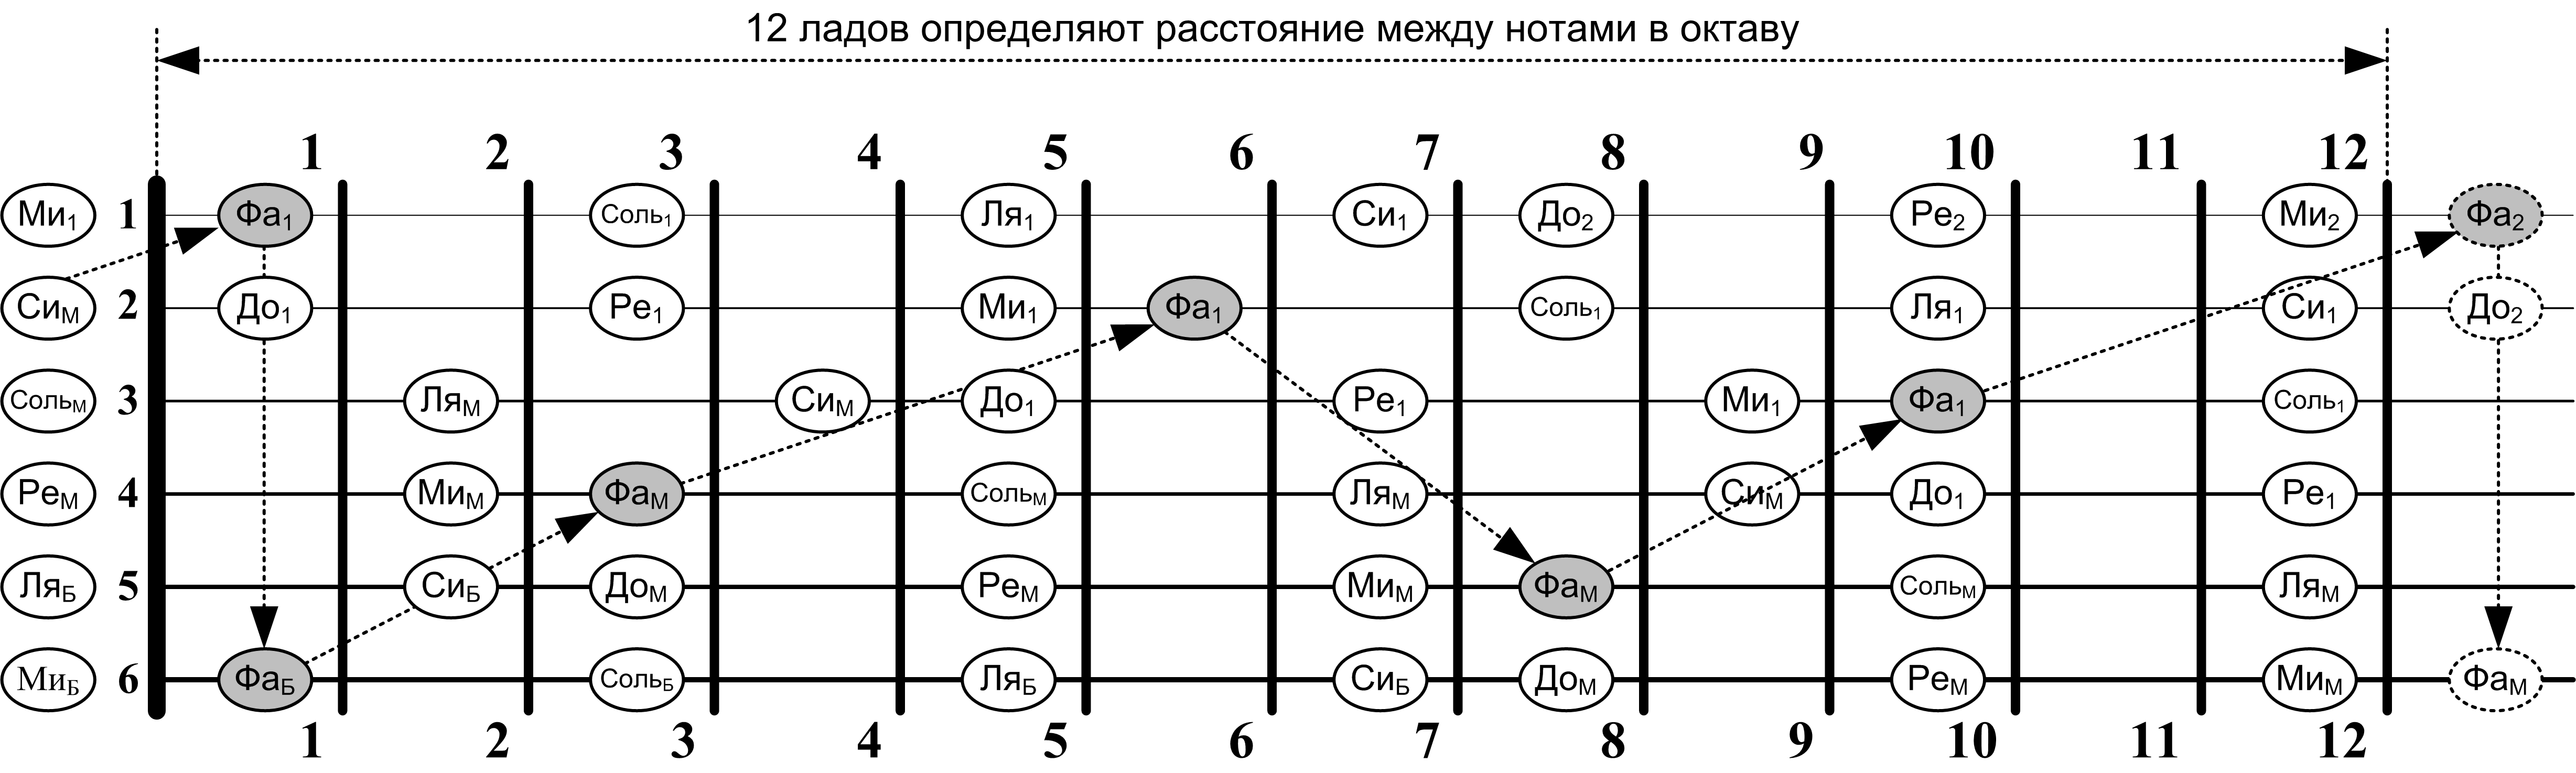
\includegraphics[width=\textwidth]{fig/notes-on-griph-ru} 
    \caption{Ноты на грифе RU\index{нота!расположение на грифе}}\label{fig:guitar:notes-on-griph-ru}
\end{figure} 

Гитаристы очень часто сталкиваются с латинскими обозначениями нот, поэтому на рисунке \ref{fig:guitar:notes-on-griph-lat} приведено все то же самое, что и на рисунке \ref{fig:guitar:notes-on-griph-ru}, только в латинских обозначениях.

\begin{figure}[!ht]
    \centering
    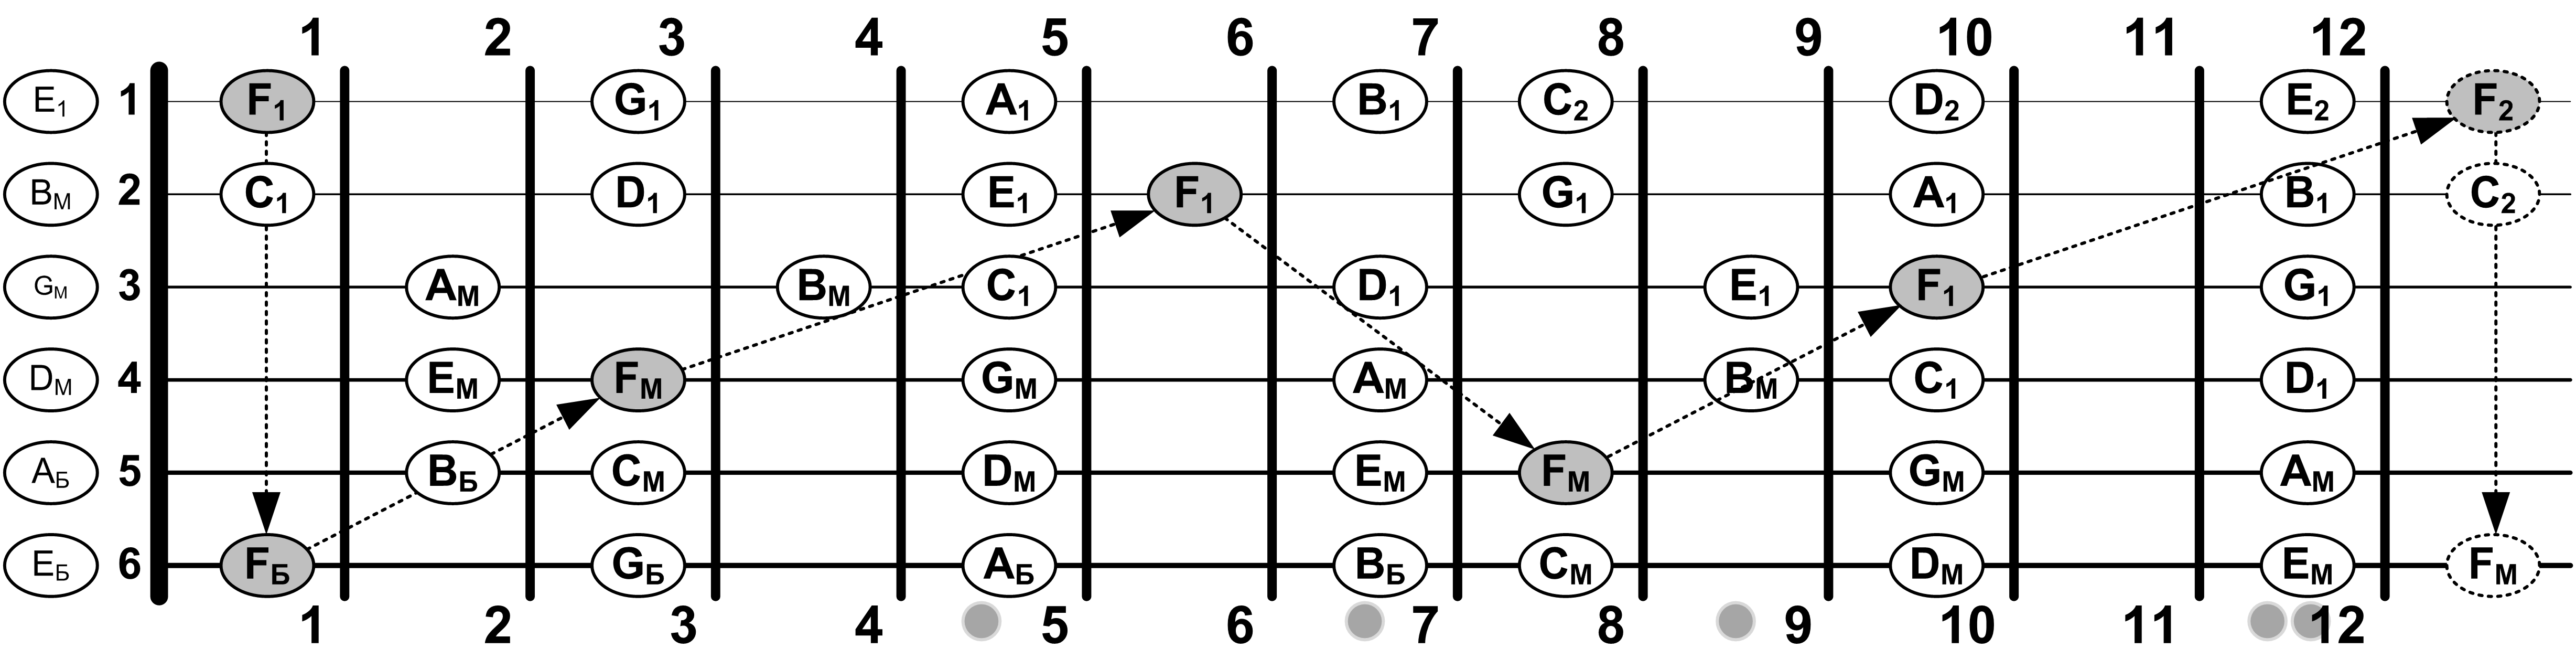
\includegraphics[width=\textwidth]{fig/notes-on-griph-lat} 
    \caption{Ноты на грифе EN\index{нота!расположение на грифе}}\label{fig:guitar:notes-on-griph-lat}
\end{figure} 

Чтобы было проще работать с нотной записью гитарной музыки, приведу также рисунки, соотносящие нотоносец и гриф.

На рисунке \ref{fig:guitar:lad-by-notes} горизонтально изображен нотоносец, а вертикально, поперек линий нотоносца --- струны. Допустим, нам нужна нота СОЛЬ малой октавы. Она пишется на второй линии нотоносца, поэтому смотрим на каких ладах эта линия пересекает линии струн: десятый лад пятой струны, пятый лад четвертой и нулевой лад третьей струны. Лады промежуточных нот не подписаны в целях экономии места, но несложно вычислить, что, например, СОЛЬ-диез малой октавы будет находится на одиннадцатом ладу пятой струны, шестом ладу четвертой и первом ладу третьей струны.
 
\begin{figure}[!ht]
    \centering
    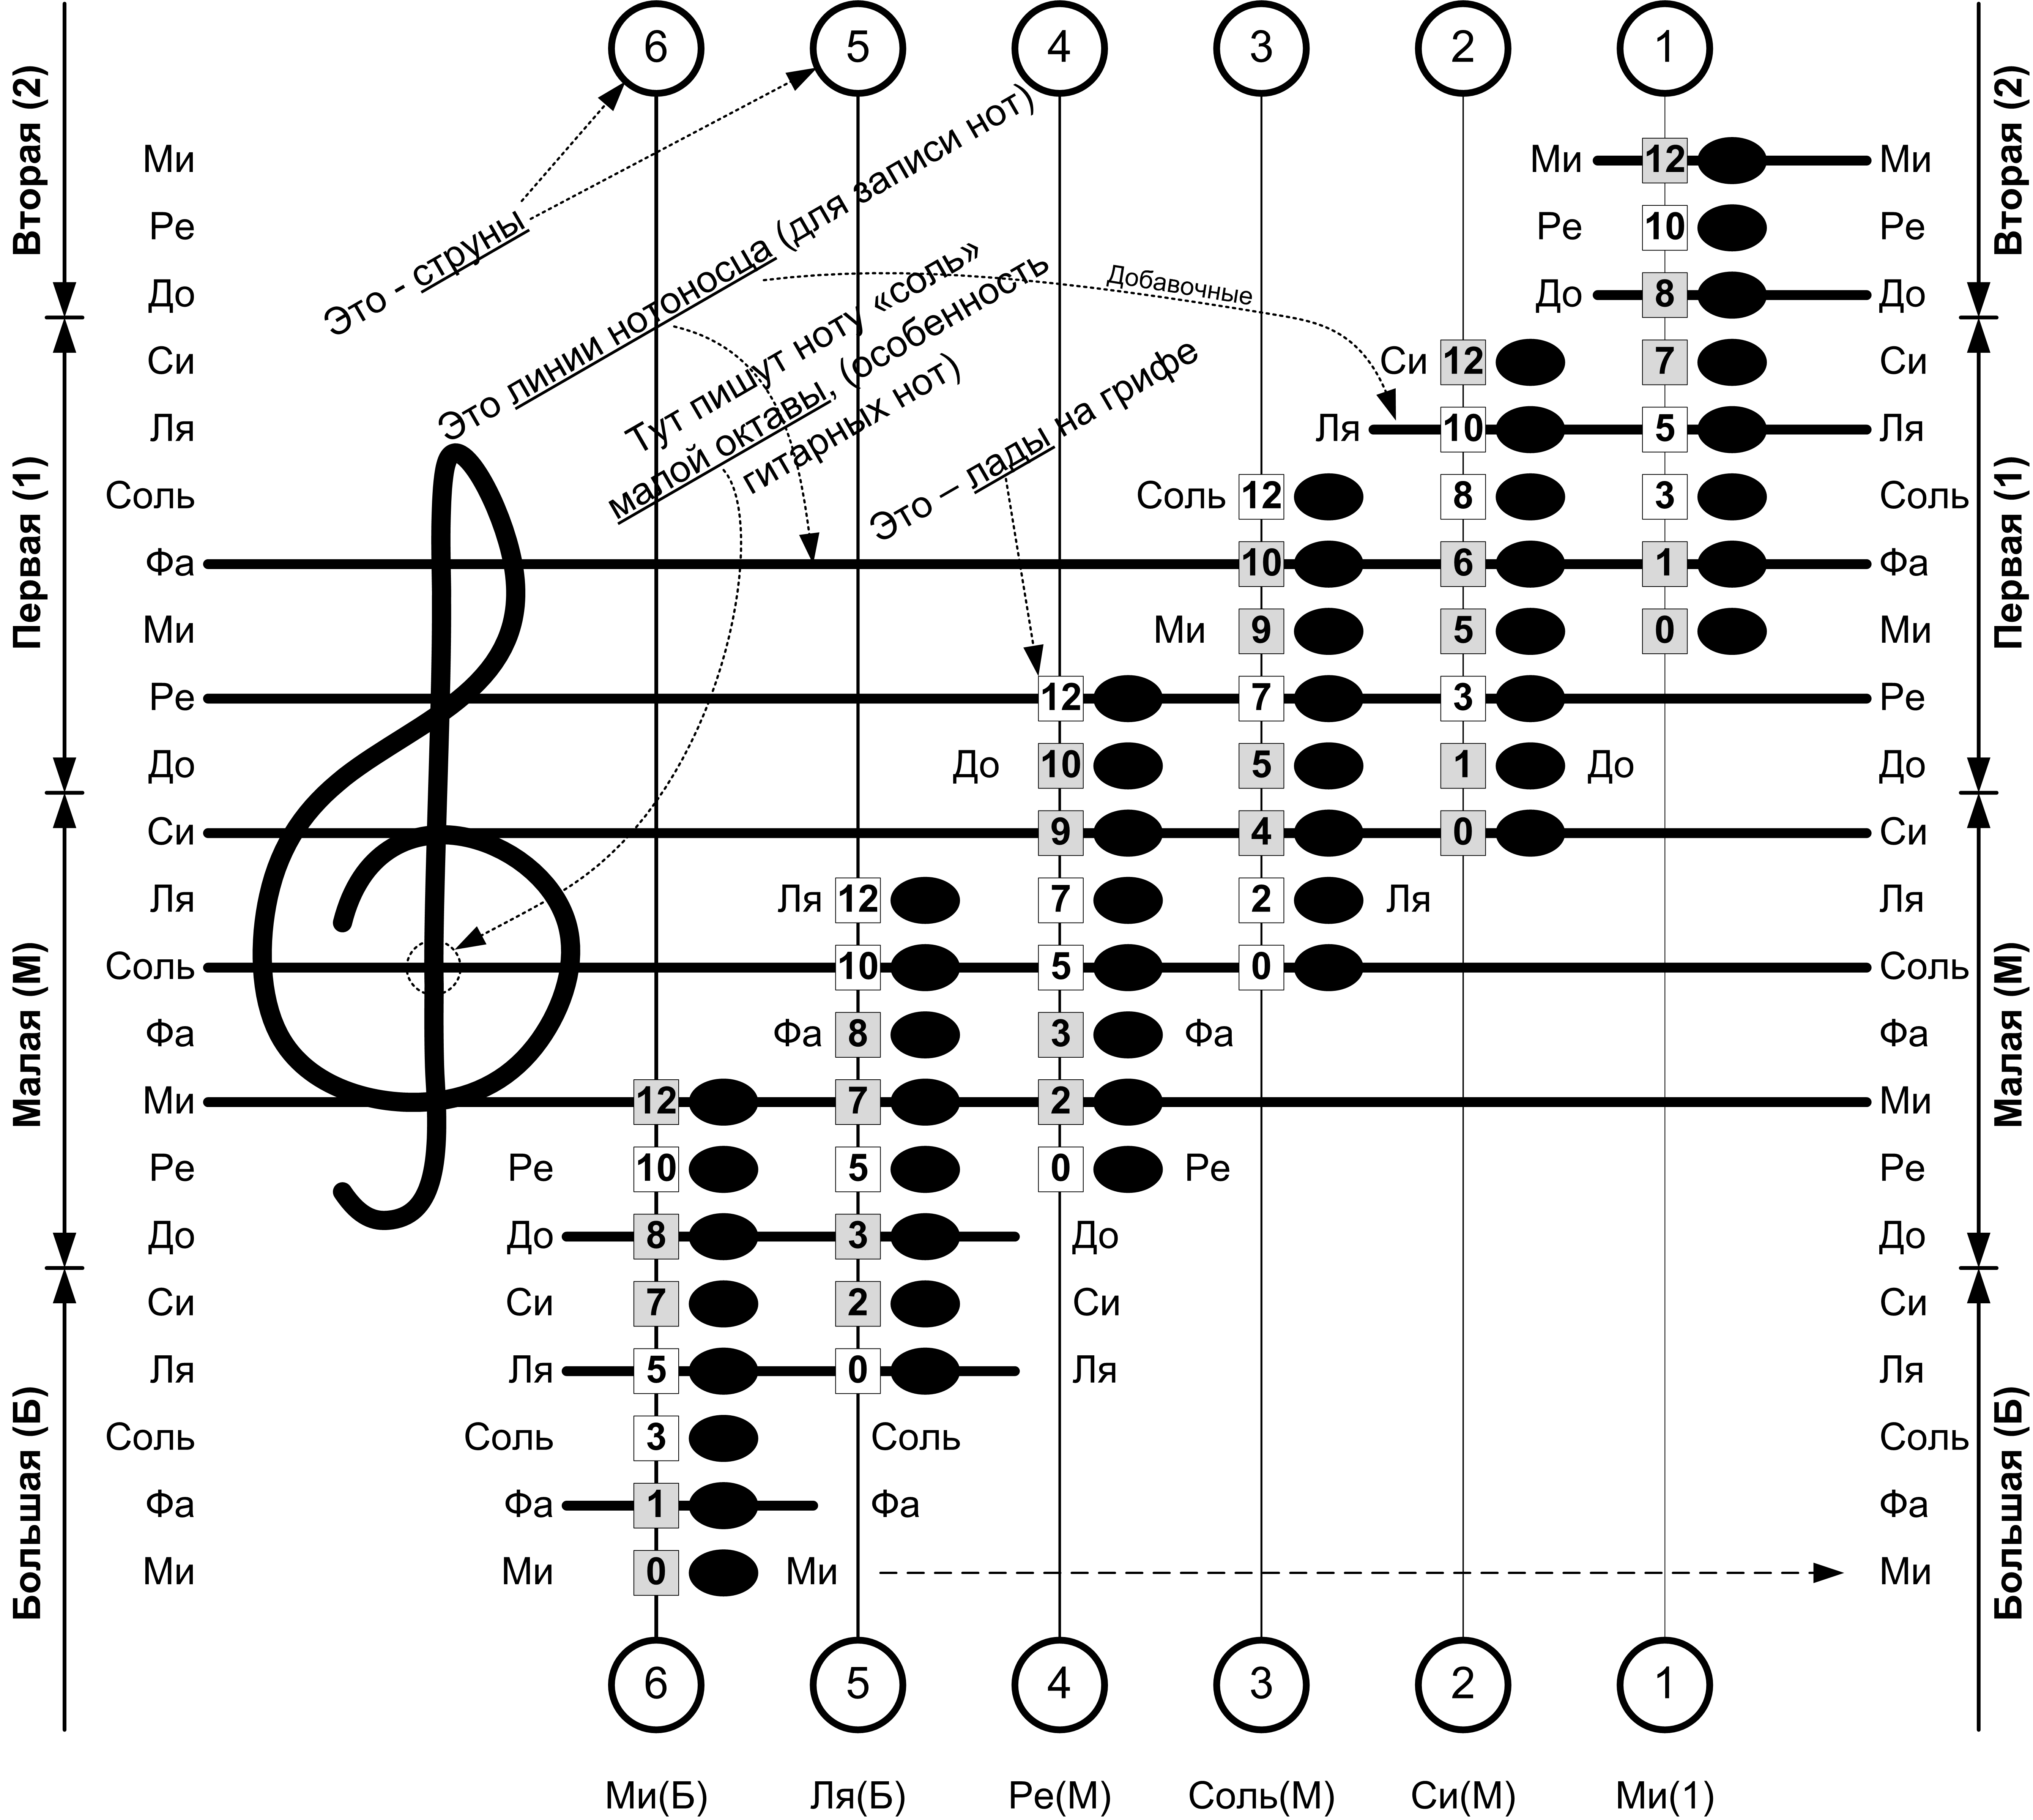
\includegraphics[width=\textwidth]{fig/lad-by-notes} 
    \caption{Ноты на грифе (гриф поперек нотоносца)\index{нота!расположение на грифе}}\label{fig:guitar:lad-by-notes}
\end{figure} 

На рисунке \ref{fig:guitar:lad-by-griph} горизонтально изображен не только нотоносец, но и струны. Например, спустившись по пунктирной линии от ноты СОЛЬ малой октавы, сделаем те же выводы, что и ранее о положении этой ноты на грифе гитары. 

\begin{figure}[!ht]
    \centering
    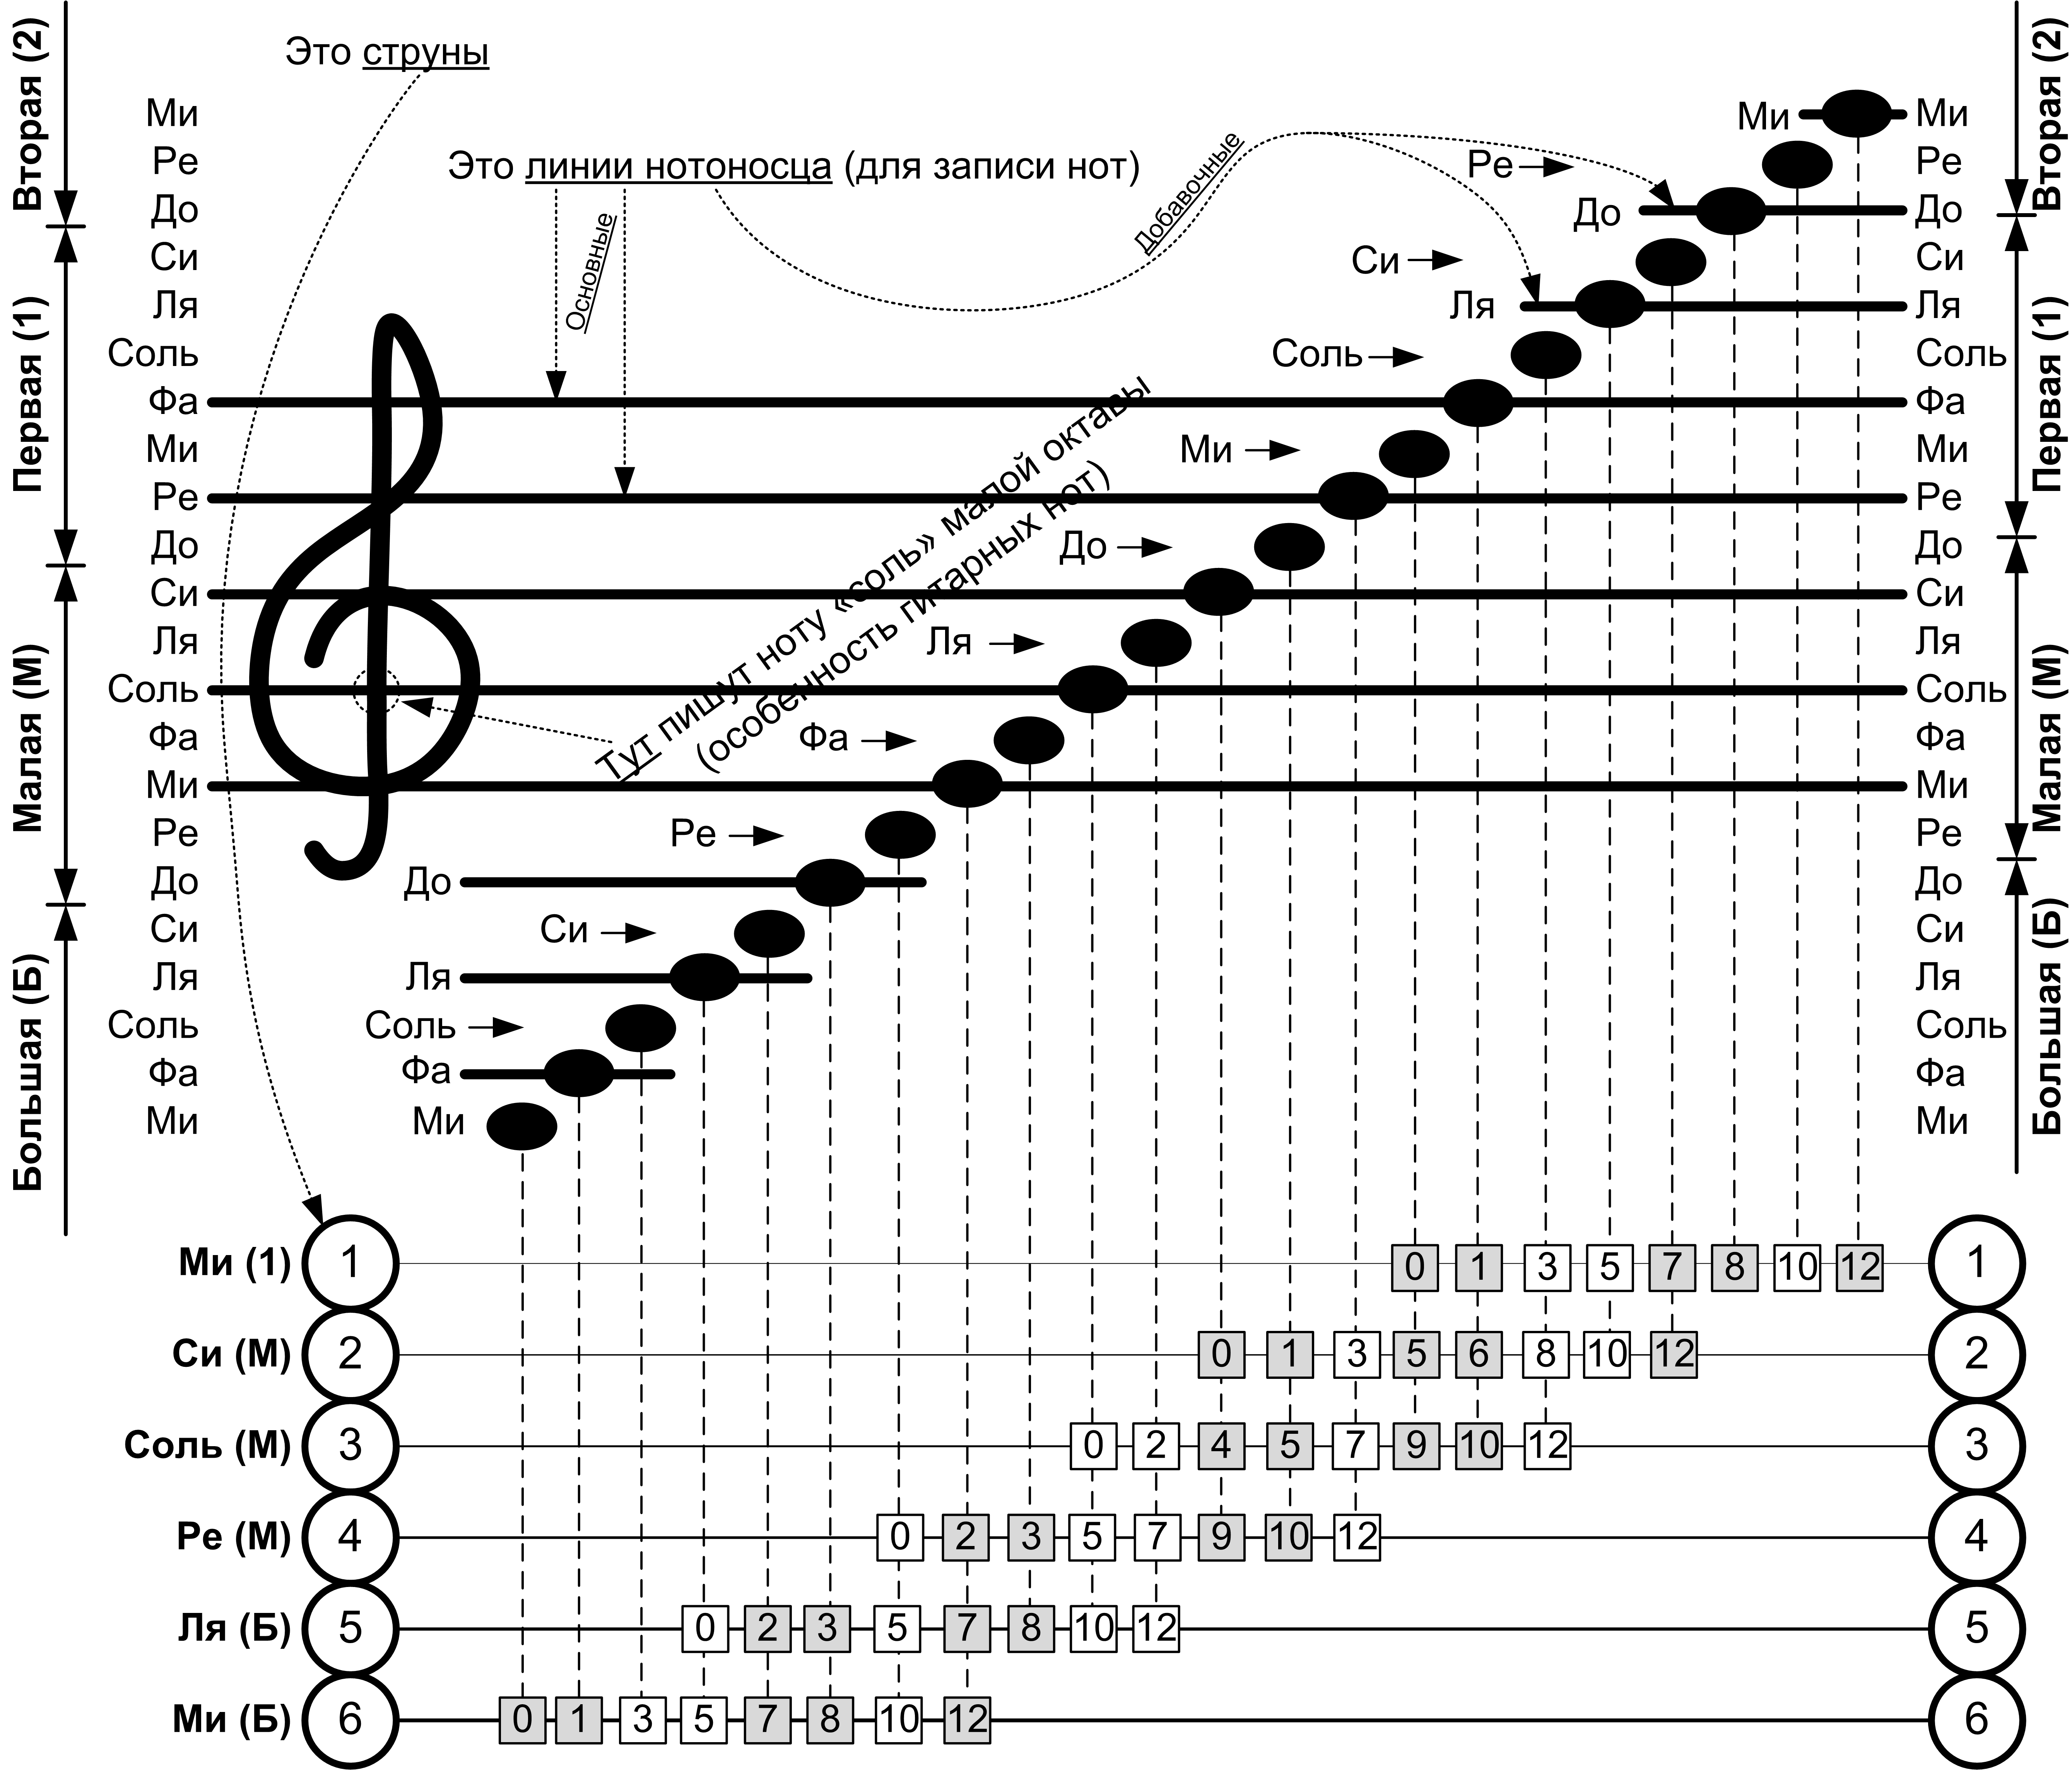
\includegraphics[width=\textwidth]{fig/lad-by-griph} 
    \caption{Ноты на грифе (гриф вдоль нотоносца)\index{нота!расположение на грифе}}\label{fig:guitar:lad-by-griph}
\end{figure} 

Стоит отметить, что на самом деле гриф 12-м ладом не заканчивается, и на всех приведенных справочных рисунках счет ладов можно было бы продолжить. Но, как уже было сказано, в процессе обучения ценность этих рисунков упадет до нуля, а на начальном этапе 12 ладов --- более, чем достаточно.

Надеюсь, вы поняли, чем гитара отличается от рояля? Верно: на гитаре \emph{одну и ту же} ноту можно найти в нескольких местах!
